\lstset{style=Python,basicstyle=\ttfamily\tiny}

\fboxsep=.6pt

% default settings for listings
\lstset{style=python}

\title[Grundlagenfach]{Informatik, Grundlagenfach}

\subtitle{Semesterprogramm}

\author[Blum, Cyril] % (optional)
{Cyril Blum}

\institute[KLW] % (optional)
{
    Fachschaft Informatik\\
    Kantonsschule im Lee
}

\date[\today] % (optional)

\logo{
\includegraphics[width=2cm]{Logos/LeeLogo}}

\titlegraphic{\vspace{-.7cm}\includegraphics[width=\textwidth]{"Grundlagen_Info/06_Datenbanken/Figures/title-emojis"}}

\frame{\titlepage}
\section{Einleitung}
\begin{frame}{Einleitung}
    \begin{itemize}[<+->]
        \item[\faCheckSquare] Themenübersicht
        \item[\faCheckSquare] Lernziele
        \item[\faCheckSquare] Semesterplan
        \item[\faCheckSquare] Vorstellung
        \item[\faCheckSquare] Grundwerte \& Regeln
        \item[\faCheckSquare] Benotung
        \item[\faCheckSquare] Fragen
    \end{itemize}
\end{frame}
\section{Themenübersicht}

\begin{frame}[fragile]{Themenübersicht}{Programmieren}
    \begin{center}
        \begin{minipage}{.4\textwidth}
            \begin{lstlisting}[escapechar=!]
import turtle as t

for _ in range(10):   
    for _ in range(4):
        t.fd(100)
        t.rt(360 / 4) 
    t.rt(360 / 10)
    
t.done()
\end{lstlisting}
        \end{minipage}\hfill\begin{minipage}{.4\textwidth}
            \begin{figure}[H]
                \centering
                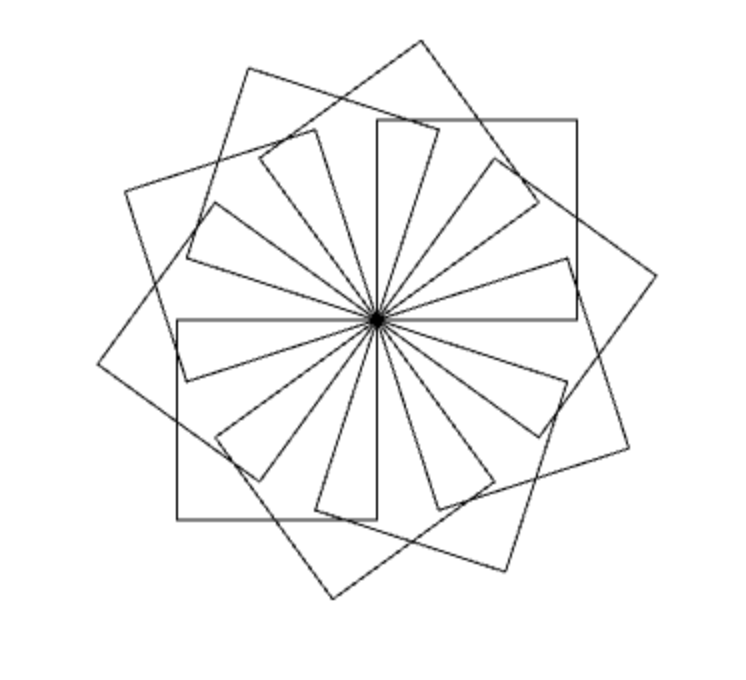
\includegraphics[width=\textwidth]{Grundlagen_Info/00_Programmieren/Figures/viereck_blume}
            \end{figure}
        \end{minipage}
    \end{center}
    \only<2->{
    \begin{center}
        \textit{Program or be programmed}  $\rightarrow$ nicht nur Apps konsumieren, sondern sich seine eigene Welt gestalten!
    \end{center}}
    \only<3->{
    \begin{center}
        \textit{Was würden Sie gerne selbst programmieren?}
    \end{center}}

\end{frame}

\begin{frame}[fragile]{Themenübersicht}{Programmieren}
    \begin{minipage}{.5\textwidth}
        \begin{figure}[H]
            \centering
            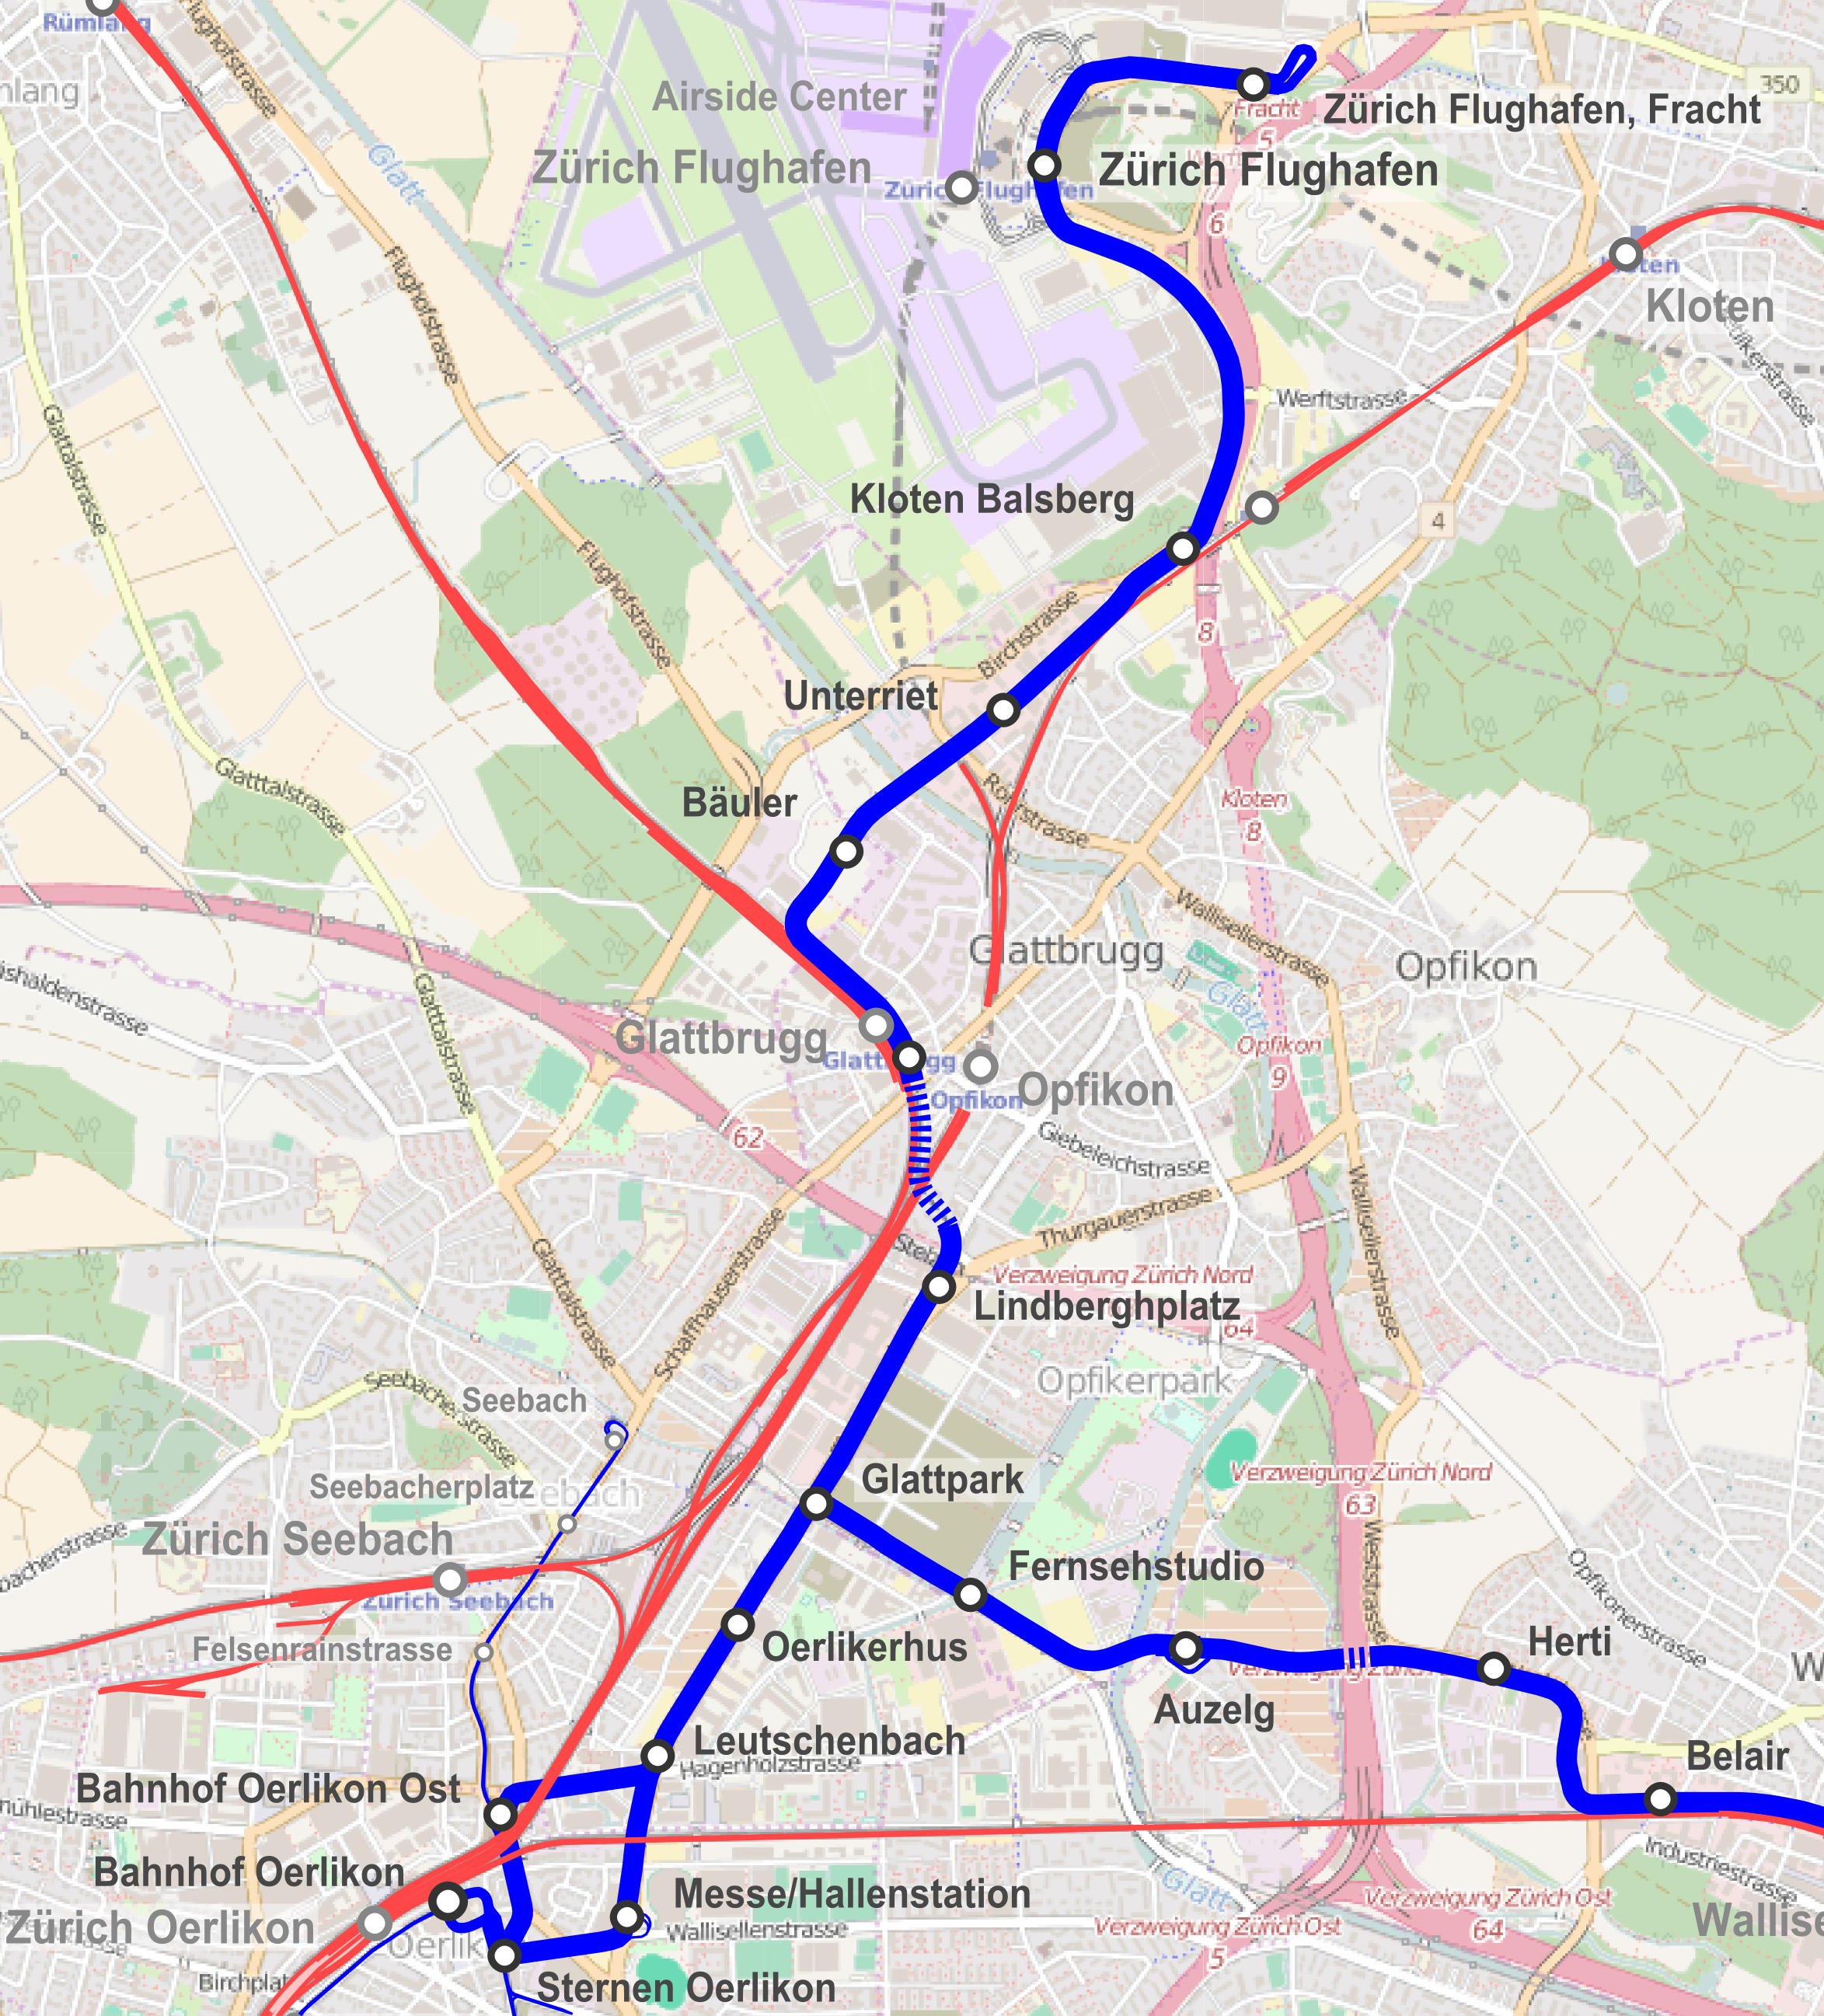
\includegraphics[width=.8\textwidth]{Grundlagen_Info/00_Programmieren/Figures/Glattalbahn_vbg}
        \end{figure}
        \begin{lstlisting}
stationen = ["Sternen", "Messe", "Leutschenbach", "Oerlikerhus", "Glattpark", "Lindbergh", "Glattbrugg", "Bäuler", "Unterriet", "Kloten", "Flughafen", "Flughafen Fracht"]
dauer = [0, 60, 122, 185, 241, 363, 543, 603, 666, 729, 786, 845]
\end{lstlisting}
    \end{minipage}
    \begin{minipage}{.05\textwidth}
        $\Rightarrow$
    \end{minipage}
    \begin{minipage}{.3\textwidth}
        \begin{figure}[H]
            \centering
            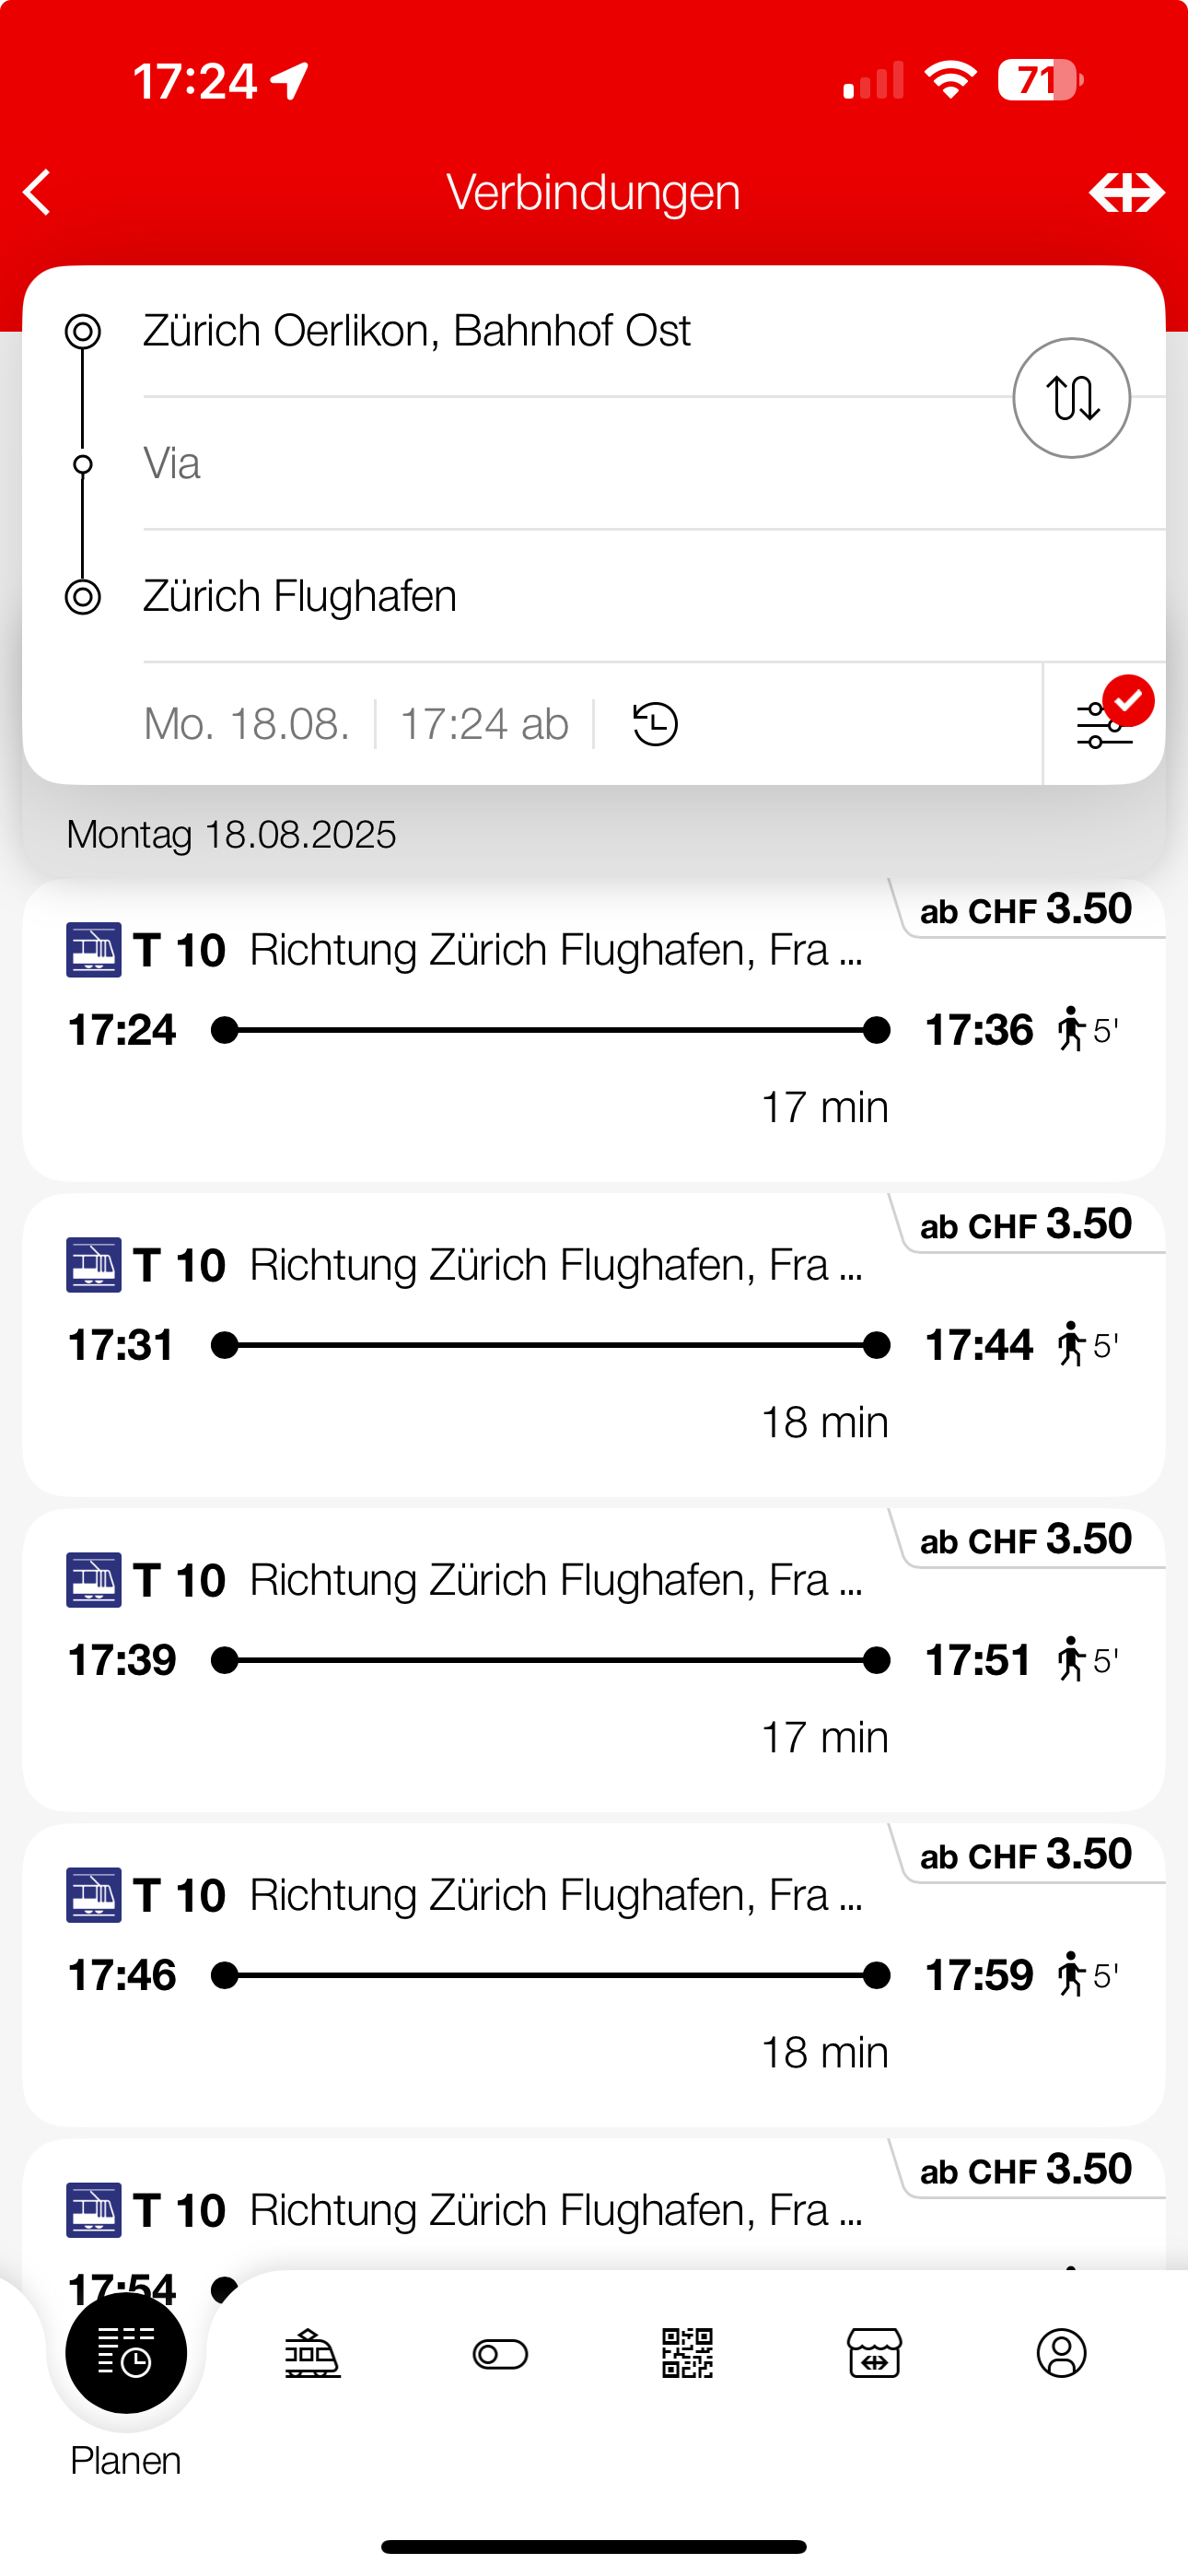
\includegraphics[width=\linewidth]{Grundlagen_Info/00_Programmieren/Figures/tram-sbb.jpeg}
        \end{figure}
    \end{minipage}
\end{frame}

\begin{frame}[fragile]{Themenübersicht}{Kodierungen}
    \begin{center}
        \textit{Ohne Kodierungen gäbe es keine Emojis, TikToks oder YouTube.} $\rightarrow$ Wo begegnen Ihnen Kodierungen im Alltag?
    \end{center}
    \begin{figure}[H]
        \centering
        \begin{subfigure}{.49\textwidth}
            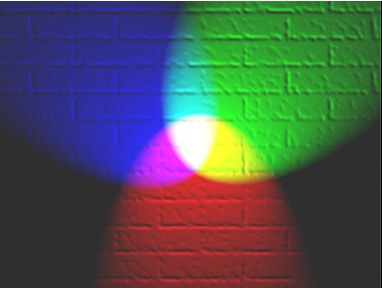
\includegraphics[width=\textwidth]{Grundlagen_Info/13_ZahlendarstellungenUndKodierungen/Figures/rgb-farbmischung-1}
        \end{subfigure}
        \begin{subfigure}{.49\textwidth}
            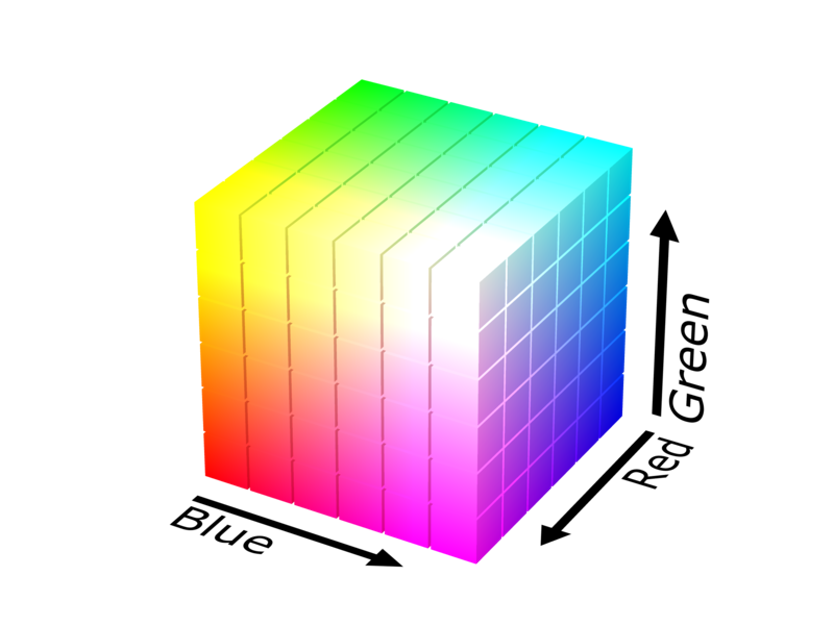
\includegraphics[width=\textwidth]{Grundlagen_Info/13_ZahlendarstellungenUndKodierungen/Figures/rgb-farbmischung-2}
        \end{subfigure}
    \end{figure}
    $\rightarrow$ Jede Farbe kodiert zwischen 0 und 255!
    \only<2->{
        \red{11111111}\green{00000000}\blue{00000000} = \#\red{FF}\green{00}\blue{00} = \red{255}, \green{0}, \blue{0} = reines Rot\\

        \red{10000000}\green{10000000}\blue{10000000} = \#\red{80}\green{80}\blue{80} = \red{128}, \green{128}, \blue{128} = grau}


\end{frame}

\begin{frame}{Farben}{Themenübersicht}{Kodierungen}
    \begin{figure}[H]
        \centering
        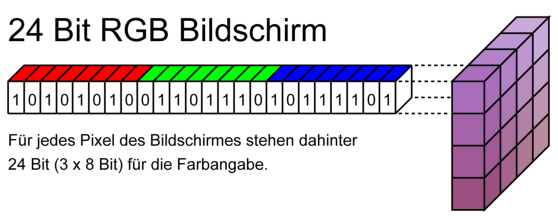
\includegraphics[width=\linewidth]{Grundlagen_Info/13_ZahlendarstellungenUndKodierungen/Figures/colordepth}
    \end{figure}
\end{frame}

\begin{frame}{Themenübersicht}{Kodierungen}
    \begin{table}[H]
        \footnotesize
        \centering
        \begin{tabular}{@{}l|rr|l@{}}
            \toprule
            \textbf{Masseinheit} & \multicolumn{2}{l|}{\textbf{Dezimalsystem}} & Grössenordnung                                   \\ \midrule
            KB (Kilobyte)        & $10^3$ B(yte)                               & 1'000 B             & eine Text-Datei            \\
            MB (Megabyte)        & $10^6$ B                                    & 1'000'000 B         & eine Musik-Datei           \\
            GB (Gigabyte)        & $10^9$ B                                    & 1'000'000'000 B     & eine Video-Datei           \\
            TB (Terabyte)        & $10^{12}$ B                                 & 1'000'000'000'000 B & kleiner Firmen-Server      \\
            PB (Petabyte)        & $10^{15}$ B                                 & ...                 & Facebook-Server            \\
            EB (Exabyte)         & $10^{18}$ B                                 & ...                 & alle CERN-Daten            \\
            ZB (Zettabyte)       & $10^{21}$ B                                 & ...                 & alle Daten ($\sim$ 100 ZB) \\
            YB (Yottabyte)       & $10^{24}$ B                                 & ...                 & $\sim$ 2030?               \\ \bottomrule
        \end{tabular}
        \caption*{Gängige Daten-Grössenordnungen in der Informatik}
    \end{table}
    \only<2->{
        \begin{center}
            Wie nennt man ein \enquote{Megagramm} geläufiger?
        \end{center}}
\end{frame}

\begin{frame}[label=schemakrypto]{Themenübersicht}{Kryptologie}
    \begin{figure}[H]
        \centering
        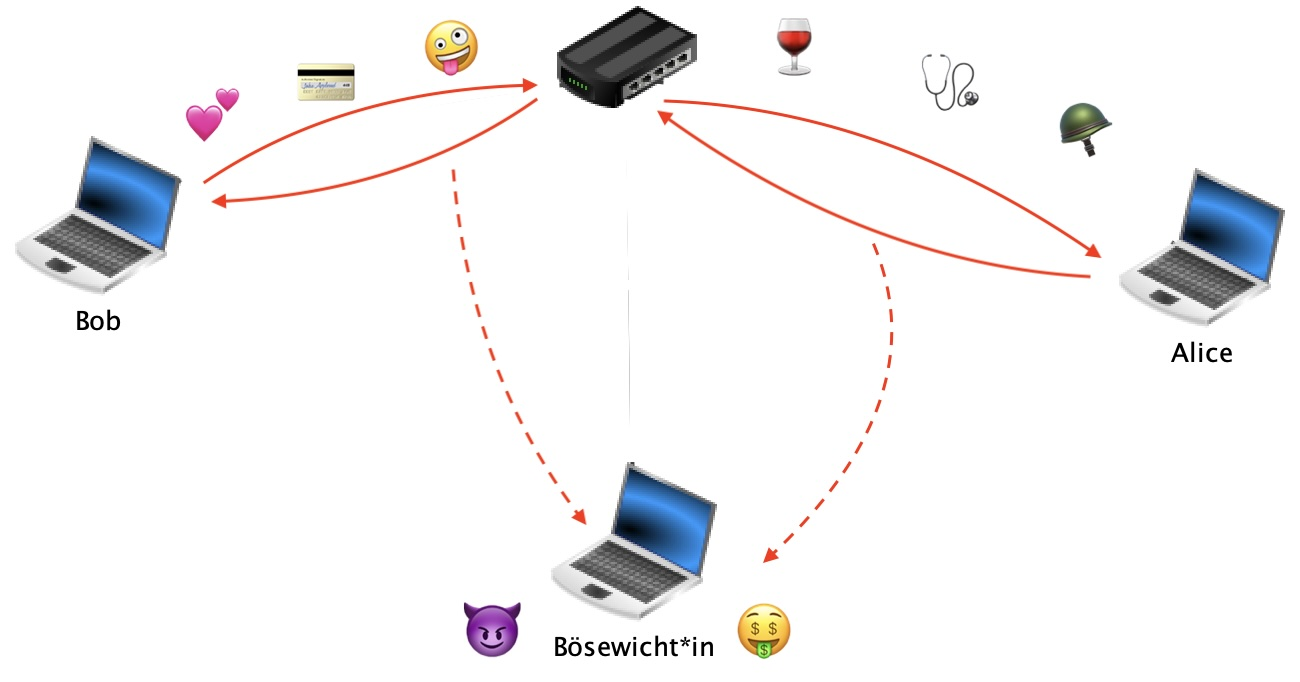
\includegraphics[width=\linewidth]{Grundlagen_Info/03_Kryptologie/Figures/filius-annotated}
        \begin{center}
            \only<1>{Was machen Sie alles im Internet?
            }
            \only<2>{
                \large Z.B.: Sie schreiben eine Nachricht an Ihr \emoji{two-hearts}...\\
                ...und ich kann alles mitlesen! \emoji{teacher}}
        \end{center}
    \end{figure}
    \begin{center}
        Wer von Ihnen würde mir Zugriff auf all Ihre Chats, Daten und Fotos gewähren?
    \end{center}

\end{frame}

\begin{frame}{Themenübersicht}{Datenintegrität}
    \begin{center}
        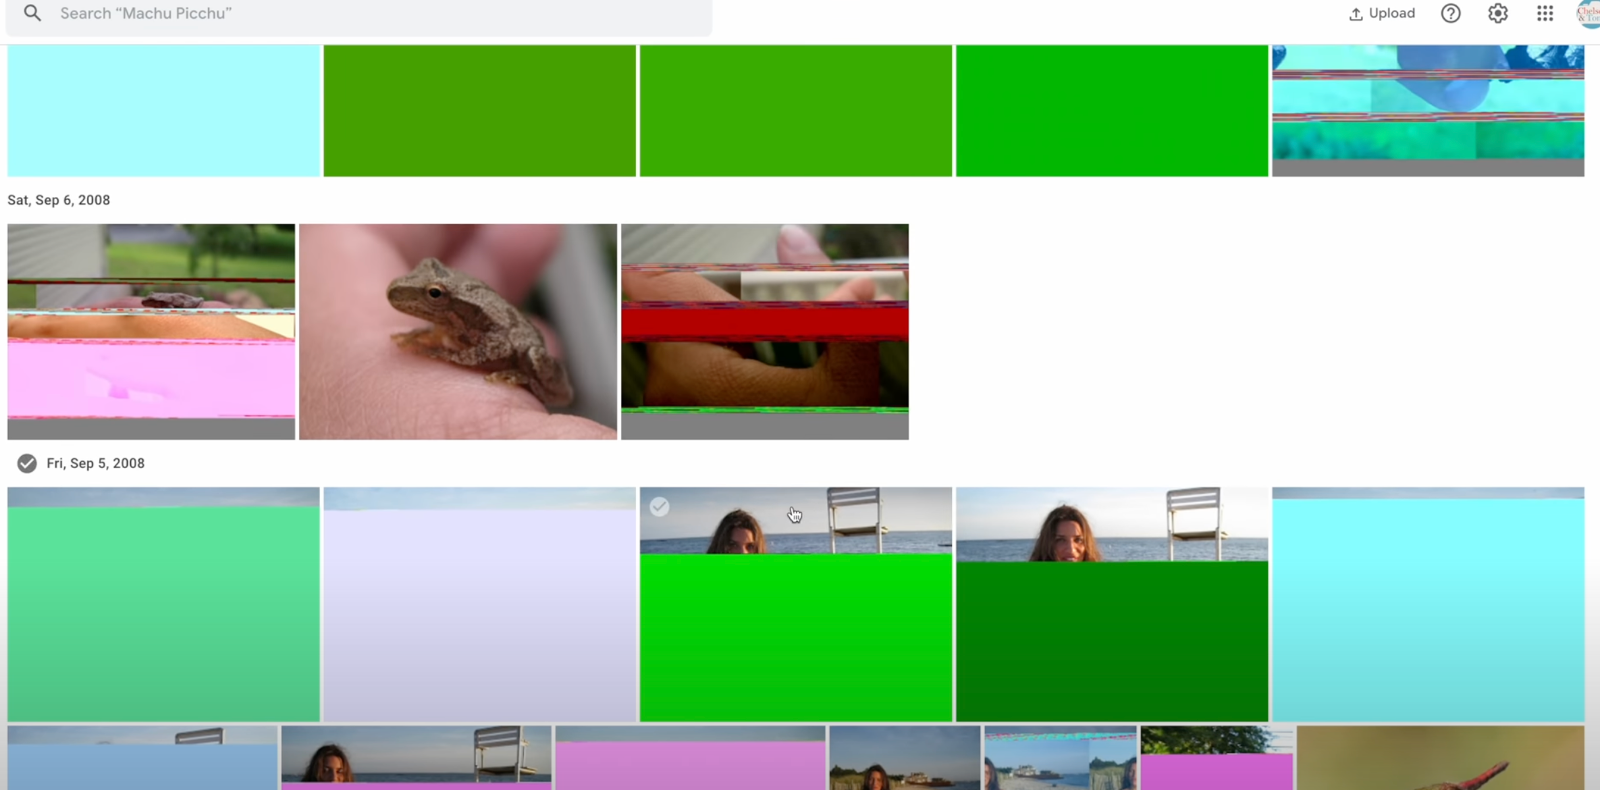
\includegraphics[width=\textwidth]{Grundlagen_Info/05_Datenintegritaet/Figures/bitrot.png}
    \end{center}
    \begin{center}
        Haben Sie schon mal einen Datenfehler bemerkt?
    \end{center}
\end{frame}

\begin{frame}{Themenübersicht}{Datenintegrität}
    \begin{center}
        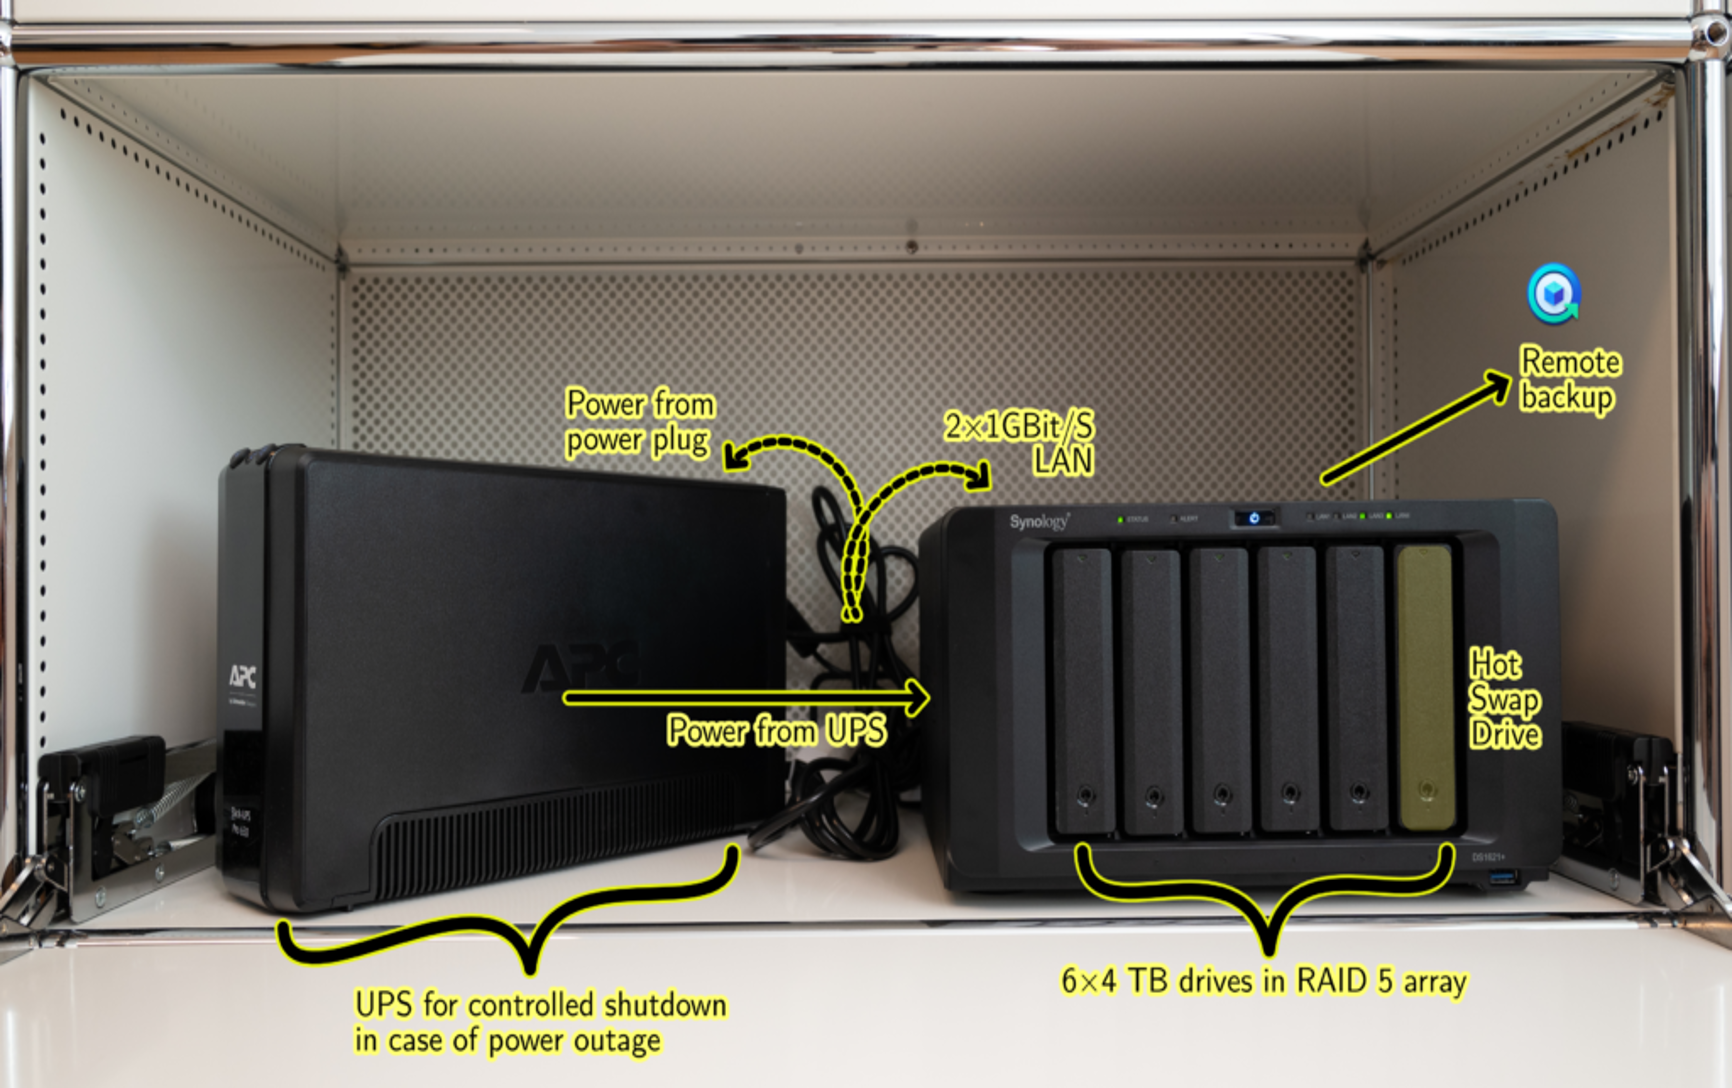
\includegraphics[width=.9\textwidth]{Grundlagen_Info/05_Datenintegritaet/Figures/NAS.png}
    \end{center}
\end{frame}

\begin{frame}{Themenübersicht}{Netzwerke}
    \begin{figure}[H]
        \centering
        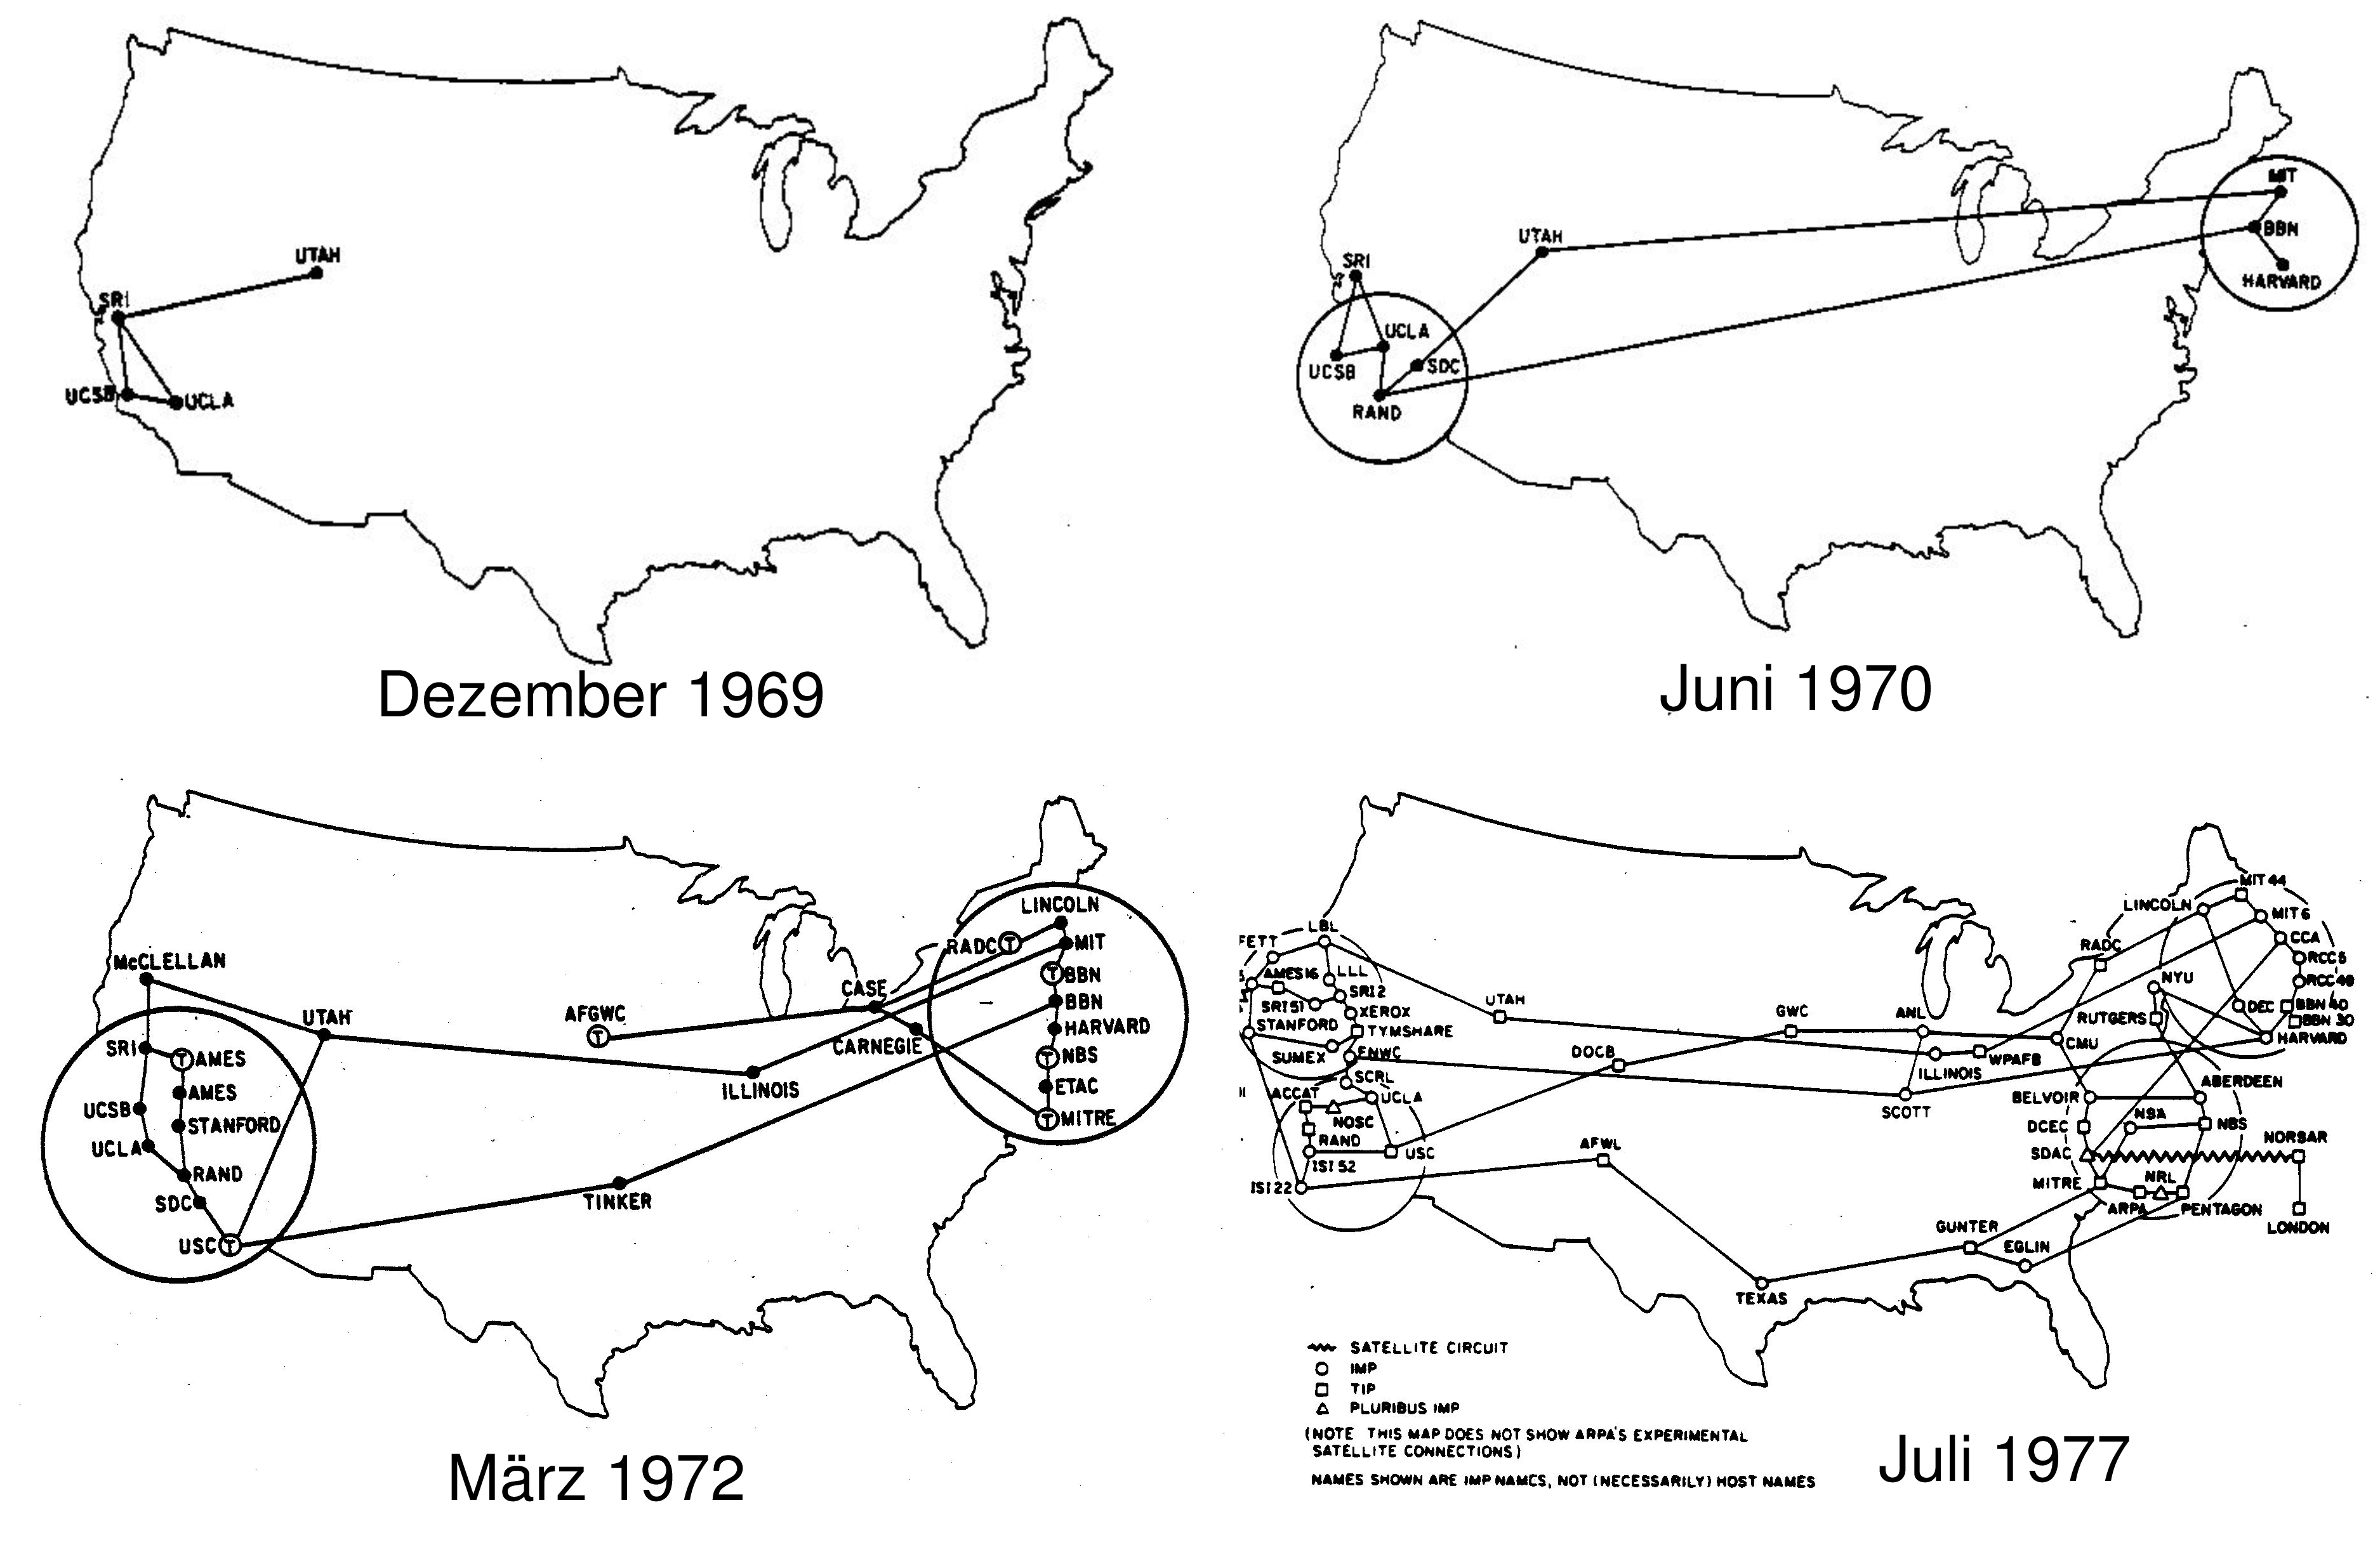
\includegraphics[width=0.7\linewidth]{Grundlagen_Info/07_Netzwerke/Figures/arpanet.png}
    \end{figure}
\end{frame}

\begin{frame}{Themenübersicht}{Netzwerke}
    \begin{figure}[H]
        \centering
        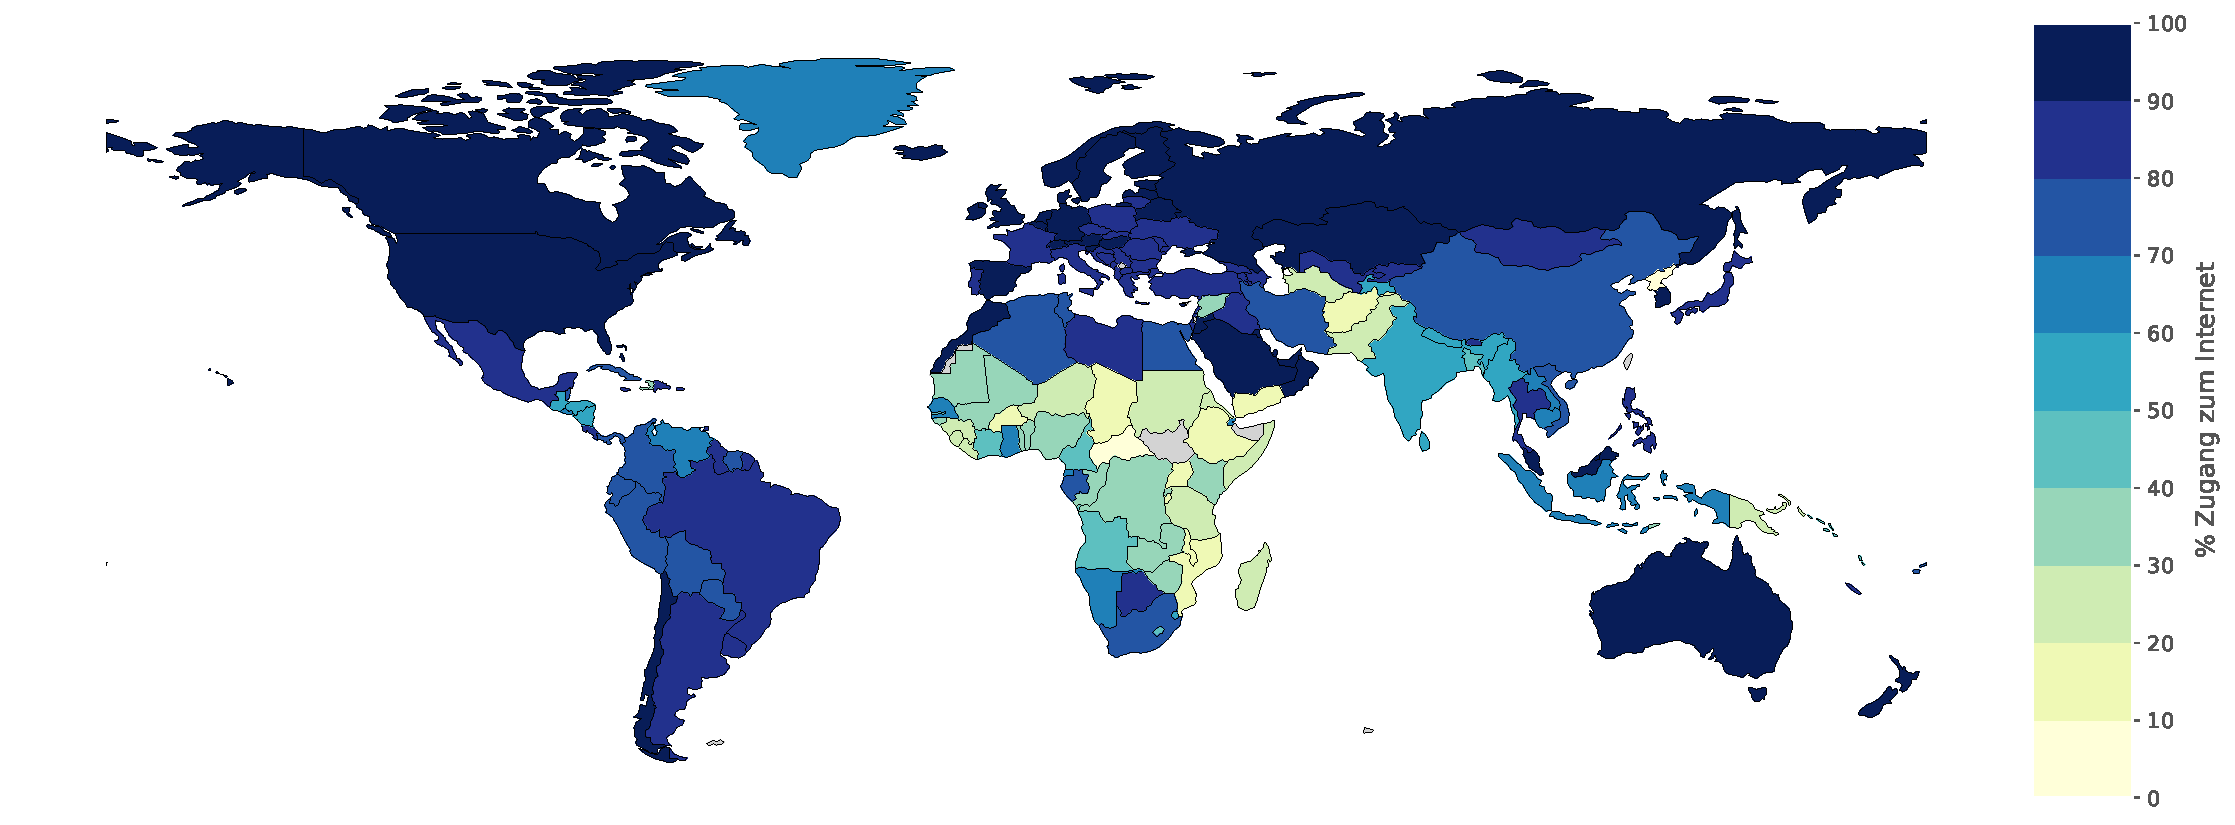
\includegraphics[width=\linewidth]{Grundlagen_Info/07_Netzwerke/Figures/internet_use_map_2024}
    \end{figure}
\end{frame}

\begin{frame}{Themenübersicht}{Netzwerke}
    \begin{figure}[H]
        \centering
        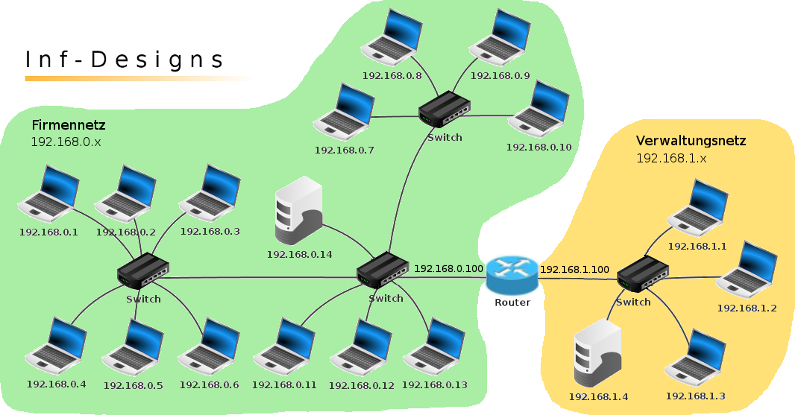
\includegraphics[width=\linewidth]{Grundlagen_Info/07_Netzwerke/Figures/subnets}
    \end{figure}
\end{frame}

\begin{frame}{Themenübersicht}{AI und Machine Learning}
    \begin{columns}
        \column{0.5\textwidth}
        \begin{itemize}
            \item Beispiel: Note über Lernaufwand und Schlaf
            \item Erklärung:
                  \begin{itemize}
                      \item $x_1$: Lernaufwand
                      \item $x_2$: Schlaf
                      \item $y$: Note
                  \end{itemize}
        \end{itemize}
        \begin{block}{Formeln}
            \begin{itemize}[<+->]
                \item Einfache lineare Regression:
                      \[\begin{aligned}
                              y & = \textcolor{red}{q} + \textcolor{blue}{m}x        \\
                                & = \textcolor{red}{a_0} + \textcolor{blue}{a_1} x_1
                          \end{aligned}\]
                \item Multiple lineare Regression:
                      \[\begin{aligned}
                              y = & \textcolor{red}{a_0} + \textcolor{blue}{a_1} x_1 + a_2x_2 + a_3 x_3 \\
                                  & + \
                              cdots + a_n x_n
                          \end{aligned}\]
            \end{itemize}
        \end{block}
        \column{0.65\textwidth}
        \begin{figure}[H]
            \centering
            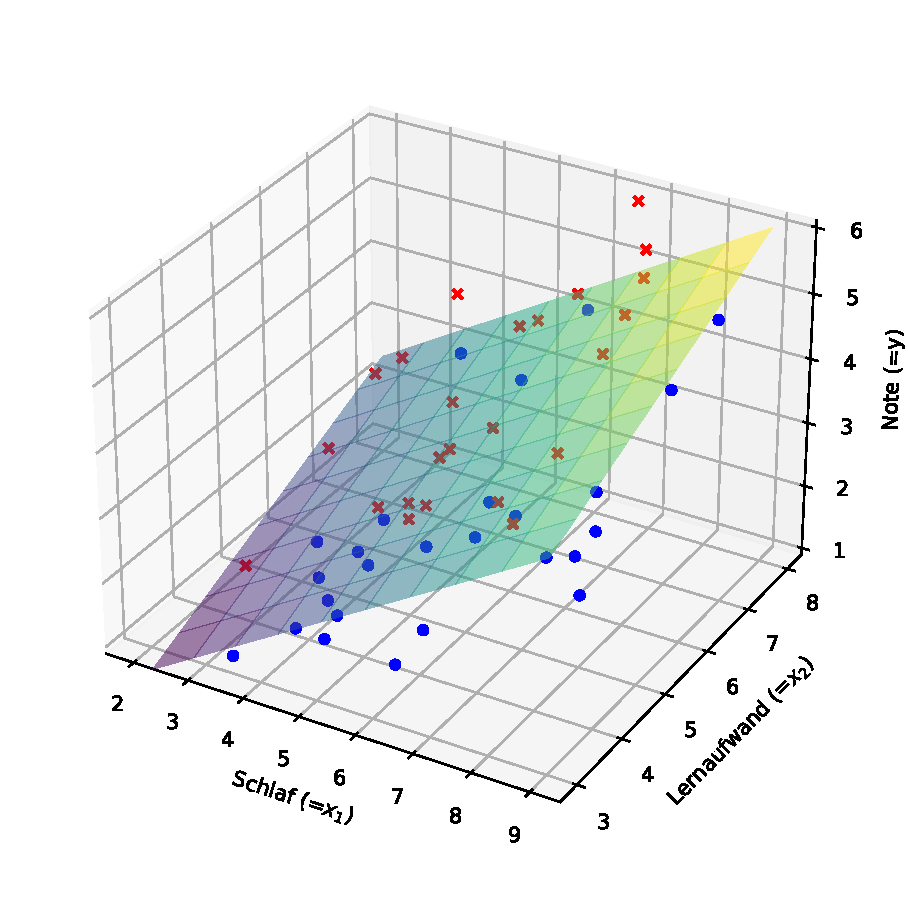
\includegraphics[width=\textwidth]{Grundlagen_Info/10_KI_und_Algorithmen/Figures/linreg_3d.pdf}
        \end{figure}
    \end{columns}
\end{frame}

\begin{frame}{Themenübersicht}{AI und Machine Learning}
    \begin{figure}[H]
        \begin{tikzpicture}[transform shape, ->, >=stealth', node distance=4cm, thick,
                website/.style={rectangle, draw, minimum width=2.5cm, minimum height=1cm, align=center}]

            \node[website] (moodle) {\texttt{moodle.ch}};
            \node[website] (intranet) [right of=moodle] {\texttt{intranet.kzn.ch}};
            \node[website] (yt) [below of=intranet] {\texttt{youtube.com}};
            \node[website] (20min) [below of=moodle] {\texttt{20minuten.ch}};

            \onslide<2>{
                \path[->]
                (moodle) edge[bend left] node[above] {0.9 (=90 \%)} (intranet)
                (moodle) edge[bend right=15] node[left] {0.1  (=10 \%)} (yt);
            }

            \onslide<3->{
                \path[->]
                (moodle) edge[bend left] node[above] {0.9} (intranet)
                (moodle) edge[bend right=15] node[left] {0.1} (yt);
            }
            \onslide<4->{
                \path[->]
                (intranet) edge[bend left] node[below] {0.8} (moodle)
                (intranet) edge node[right] {0.2} (yt);
            }
            \onslide<5->{
                \path[->] (yt.west) edge[bend left] node[below] {1} (20min.east);
            }
            \onslide<6->{
                \path[->]
                (20min.east) edge[bend left] node[above] {0.6} (yt.west)
                (20min) edge node[left] {0.4} (moodle);
            }

        \end{tikzpicture}
    \end{figure}
    \onslide<6->{
        Wenn Sie jetzt auf \texttt{moodle.ch} sind, welche Webseite möchten Sie am wahrscheinlichsten als nächstes besuchen?
    }
\end{frame}

\begin{frame}{Lernziele}
    Am Ende des Grundlagenfachs Informatik können Sie:
    \begin{itemize}[<+->]
        \item[\faCheckSquare] Komplexe Programme in \textbf{Python} schreiben
        \item[\faCheckSquare] \textbf{Daten kodieren} und effiziente \textbf{Algorithmen} zur \textbf{Datenanalyseentwickeln}
        \item[\faCheckSquare] Erklären, wie \textbf{Computer und Netzwerke} funktionieren
        \item[\faCheckSquare] Daten sicher \textbf{verschlüsseln} und übertragen
        \item[\faCheckSquare] Die Grundlagen von \textbf{Künstlicher Intelligenz} und \textbf{Machine Learning} verstehen
        \item[\faCheckSquare] Die \textbf{gesellschaftlichen Auswirkungen} der Informatik einschätzen
        \item[\faCheckSquare] \textbf{Eigene Ideen} in Informatik-Projekten umsetzen
        \item[\faCheckSquare] \textcolor{RoyalBlue}{\textbf{Mit Freude Ihren Computer nutzen, um eigene Ideen umzusetzen!}}
    \end{itemize}
\end{frame}

\begin{frame}{Themenübersicht}
    Weitere Themen sind möglich, melden Sie sich bei Interesse!
\end{frame}

\section{Semesterplan}
\begin{frame}{Semesterplan}
    \begin{center}
        \faFileExcel{} \textbf{Semesterplan} (provisorisch)
    \end{center}
\end{frame}

\section{Vorstellung}
\begin{frame}{Vorstellung}
\Wider{\begin{tikzpicture}[m/.style={draw, color=RoyalBlue, text=black, align=left, font=\tiny, fill=RoyalBlue!30, fill opacity=.3, rounded corners,text opacity=1}]
    \node[anchor=south west,inner sep=0] at (0,0) {\includegraphics[width=\textwidth]{"Private/Presentation/ch"}};
    \
    % Burgdorf
    \node[m](Burgdorf) at (5.3,4.5) {\faMapMarker{} Burgdorf};
    
    \only<2->{
	    % Bern
        \node[m](Bern) at (4.5,4.5) {\faMapMarker{} Bern\\\includegraphics[width=1cm]{"Private/Presentation/Logos/logo_gk"}};
        \draw (Burgdorf.north) edge[->, bend right=90] (Bern.north);}
    
    \only<3->{
	    % Fribourg
        \node[m](Fribourg) at (3.6,3.5) {\faMapMarker{} Fribourg\\\includegraphics[width=.7cm]{"Private/Presentation/Logos/logo unifr"}};
        \draw (Bern.south) edge[->, bend left=30] (Fribourg.east);
    }
    
    \only<4->{
    	% Lausanne
        \node[m](Lausanne) at (2.2,3) {\faMapMarker{} Lausanne\\\includegraphics[width=.7cm]{"Private/Presentation/Logos/logo epfl"}};
       	\draw (Fribourg.south) edge[->, bend left=30] (Lausanne.east);
    }  
    
    \only<5->{
        % Netherlands
        \node[m](Wageningen) at (1.5,7.5) {\faMapMarker{} Wageningen\\\includegraphics[width=1.3cm]{"Private/Presentation/Logos/logo_wur"}};    
        \draw[dashed] (Lausanne.north) edge[->, bend left=15] (Wageningen.south);
        \draw[dashed] (Wageningen.south) edge[->, bend left=15] (Lausanne.north);
    }

	\only<6->{
			 % Paris
	        \node[m](Paris) at (0,6) {\faMapMarker{} Paris\\\includegraphics[width=.9cm]{"Private/Presentation/Logos/logo_cdi"}};
	        \draw (Lausanne.west) edge[->, bend left=15] (Paris.south);
    
    }
    
	\only<7->{
	% Zürich
	        \node[m](Zurich) at (7.1,6.2) {\faMapMarker{} Zürich\\\includegraphics[width=.7cm]{"Private/Presentation/Logos/PartnerRe"}};
	        \draw (Paris.east) edge[->, bend left=15] (Zurich.west);
    
    }
    
    \only<8->{
   		% Winterthur
     	\node[m](Winterthur) at (7.5,6.8) {\faMapMarker{} Winterthur\\\includegraphics[width=1.2cm]{"Private/Presentation/Logos/Logo Kantonsschule im Lee"}};
	     \draw (Zurich.east) edge[->, bend right=30] (Winterthur.east);  
    }
    
    
\end{tikzpicture}}
\end{frame}

\begin{frame}{Interessen}
\begin{center}
\href{https://cblum.ch}{cblum.ch}
\end{center}
\end{frame}

\begin{frame}{Hauptziel}
\begin{center}
    \only<1>{\textcolor{RoyalBlue}{\faGraduationCap \textbf{Abschluss:} Maturität}}
    \only<2->{\sout{\textit{\textcolor{RoyalBlue}{\faGraduationCap \textbf{Abschluss:} Maturität}}}\\
    \textcolor{RoyalBlue}{\textbf{Spass an der Informatik und am eigenen Computer gewinnen!}}}
\end{center}
\end{frame}


\section{Grundwerte \& Regeln}
\begin{frame}{Grundwerte \& Regeln}
    \begin{overviewBox}
        \textit{Achte auf Deine Gedanken, denn es liegt in der Natur des Gedankes, Wirklichkeit zu werden.}
    \end{overviewBox}
    \begin{itemize}[<+->]
        \item[\faShoppingBag] Nutzen Sie Ihre wertvolle Zeit $\rightarrow$ Füllen Sie Ihren Rucksack
        \item[\faComments] Seien Sie \textbf{proaktiv}, fragen Sie nach
        \item[\faExclamationTriangle] Machen Sie \textbf{Fehler}, probieren Sie Dinge aus!
        \item[\faThumbsUp] Geben Sie mir \textbf{konstruktives Feedback}
    \end{itemize}
\end{frame}

\begin{frame}{Grundwerte \& Regeln}
    \begin{enumerate}
        \item Dokument bitte durchlesen
        \item Änderungen und Erweiterungen vorschlagen
        \item Dokument vorne unterschreiben
    \end{enumerate}
    Vielen Dank!
\end{frame}

\section{Benotung}
\begin{frame}{Benotung}
    \begin{enumerate}[<+->]
        \item[\faPen] Jede \textbf{schriftliche Prüfung} zähle 1 Note
        \item[\faMoneyBill] \textbf{Boni}: mündlich und Feedback an mich (kann nur positiv sein)
        \item[\faFilePdf] PDF auf Moodle, kurz lesen und danach fragen stellen
    \end{enumerate}
    \begin{center}

    \end{center}
\end{frame}

\begin{frame}{\faQuestionCircle}\Huge
    \begin{center}
        Fragen?
    \end{center}
\end{frame}